\documentclass[11pt]{article}

\usepackage[margin=1in]{geometry}
\usepackage{graphicx}
\usepackage{booktabs}
\usepackage{amsmath}
\usepackage{amssymb}
\usepackage{caption}
\usepackage{float}
\usepackage{xcolor}
\usepackage[hidelinks]{hyperref}
\usepackage{enumitem}

\captionsetup{font=small,labelfont=bf}
\setlist{nosep,leftmargin=1.4em}
\graphicspath{{figures/}}

\newcommand{\acc}[1]{\textbf{#1}}
\newcommand{\code}[1]{\texttt{#1}}

\title{\vspace{-2.0em}Working with atlas-transferred colour--texture data:\\
from colour morphospaces to an expert-in-the-loop pattern tool}
\author{Aleksandr Spiridonov}
\date{21 June 2026}

\begin{document}
\maketitle
\vspace{-1.5em}

\begin{abstract}
\noindent
We have a tool that bakes per-specimen colour textures onto a shared mean/atlas mesh, turning a set of
3D-scanned organisms into an aligned, population-scale colour--texture dataset. This report addresses the
follow-on question: \emph{how does a biologist actually work with that data?} We trace a deliberate
progression. A colour morphospace (PCA on colour composition) solves the easy, high-variance factors --- hue
clusters separate cleanly and auto-cluster correctly --- but goes no further. Subtle \emph{pattern} (stripe
count, texture) is invisible to colour, so we introduce a general, CPU-only graph-spectral / GFT descriptor
that raises the recoverable signal substantially. Yet a deeper limit remains: \emph{purely unsupervised}
discovery cannot surface low-variance, overlapping, or rare structure --- this is a property of
high-dimension--low-sample-size geometry, not a tuning failure, and a trustworthy pipeline must therefore
\emph{abstain} rather than fabricate. The productive resolution is a small amount of expert supervision. We
show that multi-label \emph{tagging} --- the expert names traits and clicks specimens that have them --- is
far more label-efficient than pairwise similarity feedback and yields a directly interpretable classifier
latent. We describe the expert-tagging tool that resulted, justifying each design choice with the underlying
experiments, and summarise the full study in an appendix.
\end{abstract}

\section{Introduction}

The upstream tool performs \emph{atlas texture transfer}: every specimen's surface colour is resampled onto a
single shared mean mesh with a common UV layout, so that a fixed face (or region) refers to the same anatomical
location across all individuals. The output is a registered $(\text{specimens} \times \text{faces} \times
\text{colour})$ tensor --- a population in correspondence. This is genuinely new data for a lab, and it invites
an obvious question that turns out to be the hard part: \emph{what analysis lets a non-technical biologist see
the population's structure, with minimal UI?}

This report follows the path the project actually took:
\begin{enumerate}
  \item \textbf{Colour only goes so far.} A colour morphospace already solves the high-variance hue factors
  (Sec.~\ref{sec:colour}); it does not touch pattern.
  \item \textbf{Pattern needs structure-aware descriptors.} Graph-spectral / GFT features on the mesh recover
  pattern that colour PCA cannot (Sec.~\ref{sec:pattern}).
  \item \textbf{Unsupervised discovery has a hard ceiling.} Even with the right descriptor, subtle/overlapping/
  rare structure is supervised-recoverable but \emph{not} unsupervised-discoverable (Sec.~\ref{sec:wall}).
  \item \textbf{Expert supervision works.} Multi-label tagging breaks the ceiling cheaply and is what we
  shipped (Secs.~\ref{sec:tag}--\ref{sec:tool}).
\end{enumerate}

\paragraph{Datasets.} We develop and validate on two populations. \emph{Fishy} is a synthetic set of
$n{=}250$ textured fish with four \emph{known} planted factors, used as ground truth: \emph{belly} hue (2
groups), \emph{tail} hue (2 groups), \emph{stripe} count (4 vs.\ 5, an 80/20 split), and rare \emph{rosy
cheeks} (5.6\%, present on only 14/250). \emph{Mussels} is a real population of $n{=}31$ scanned shell valves
with no ground truth, used to check that conclusions transfer to real, small-$n$ data. Everything is CPU-only
and assumes the unlabelled regime; ground-truth labels are used for validation only, never to colour a
user-facing plot.

\section{Colour is easy --- and already solved}
\label{sec:colour}

The existing colour morphospace (PCA on an area-weighted colour histogram, or per-region mean colour) already
recovers the high-variance colour factors essentially perfectly. On fishy, belly and tail hue land on PC1/PC2
as four clean quadrants; balanced cross-validated classification accuracy is $\approx\!1.00$ for both, and an
automatic GMM+BIC clustering of the colour plane recovers the four belly$\times$tail groups at
\acc{ARI $=0.99$} with no tuning (Fig.~\ref{fig:colour}). On the real mussels the same machinery finds an
interpretable periostracum-darkness split. \emph{This part needs no change.} The lesson that matters is the
flip side: colour PCA scores stripe at only \acc{0.64} and cheeks at \acc{0.48} ($\approx$ chance). The
high-variance axes a colour morphospace surfaces are exactly the \emph{nuisance} ones (base hue, belly/tail
colour); the biologically interesting pattern variation contributes little total variance and is buried.

\begin{figure}[H]
  \centering
  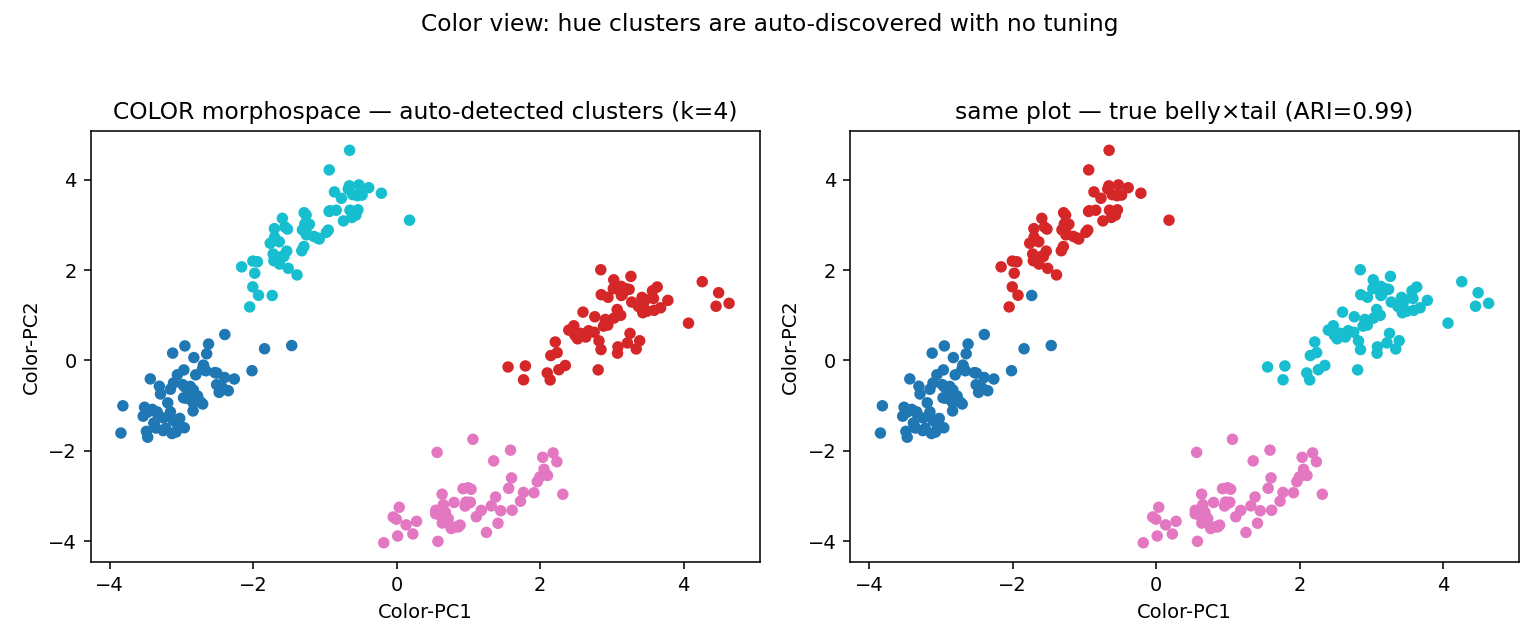
\includegraphics[width=0.86\linewidth]{fig1_color_morphospace.png}
  \caption{The colour morphospace already solves the easy factors: belly$\times$tail hue form four clean
  groups that an automatic clusterer recovers at ARI~0.99. Subtle pattern (stripe count) and the rare cheeks
  variant are \emph{not} here --- they carry little variance and stay hidden.}
  \label{fig:colour}
\end{figure}

\section{Pattern needs a structure-aware descriptor}
\label{sec:pattern}

Stripe count is a \emph{geometric}, shift-jittered feature: a colour-composition histogram is blind to it, and
even spatial colour vectors are smeared because stripe positions vary specimen-to-specimen. The fix is a
descriptor that encodes \emph{layout}, not just composition. We settled on a \textbf{graph Fourier transform
(GFT)} representation: treat each colour channel as a signal on the mesh graph and project it onto the low
eigenmodes of the mesh Laplacian (``sines and cosines on the surface''). Signed GFT coefficients are general
(no pattern-specific assumptions), mesh-intrinsic (UV/topology-independent, which matters for real meshes), and
CPU-trivial. A shared-codebook \emph{texton} histogram --- a texture vocabulary learned from the millions of
pooled local patches across all specimens --- pushes stripe a little further still.

\begin{table}[H]
  \centering
  \small
  \caption{Balanced cross-validated accuracy per factor (chance $\approx 0.5$), by descriptor. Colour PCA
  solves the hue factors but not pattern; the GFT/texton descriptors recover stripe and lift cheeks, with
  \emph{no} hand-coded body axis. Pattern is recoverable by a \emph{classifier} --- it still does not appear on
  the leading unsupervised axes (Sec.~\ref{sec:wall}).}
  \label{tab:descriptors}
  \begin{tabular}{lcccc}
    \toprule
    factor & colour PCA & GFT coeff.\ ($k{=}40$) & texton BoW & \emph{best supervised} \\
    \midrule
    belly  & 1.00 & 1.00 & 1.00 & 1.00 \\
    tail   & 1.00 & 1.00 & 1.00 & 1.00 \\
    stripe & 0.64 & 0.93 & \acc{0.97} & 0.97 \\
    cheeks & 0.48 & \acc{0.77} & 0.54 & $\sim$0.79 \\
    \bottomrule
  \end{tabular}
\end{table}

A consistent, important subtlety surfaced here and recurs throughout: \textbf{the discriminative signal lives
in the low-variance tail of the representation.} Figure~\ref{fig:dims} sweeps the number of PCA dimensions.
Colour classification saturates by $\approx\!4$ dimensions; stripe accuracy keeps climbing to
$\approx\!30$ dimensions, while a 95\%-explained-variance criterion would stop at $\approx\!12$. \emph{Explained
variance under-counts the dimensions the subtle factor needs.} This single observation justifies a core demo
choice --- keep $\approx\!24$ PCA dimensions, sized by the hardest factor, not by a variance threshold (which
would silently discard stripe). The same plot shows the wall ahead: stripe's unsupervised cluster ARI is
$\approx\!0$ at \emph{every} dimensionality.

\begin{figure}[H]
  \centering
  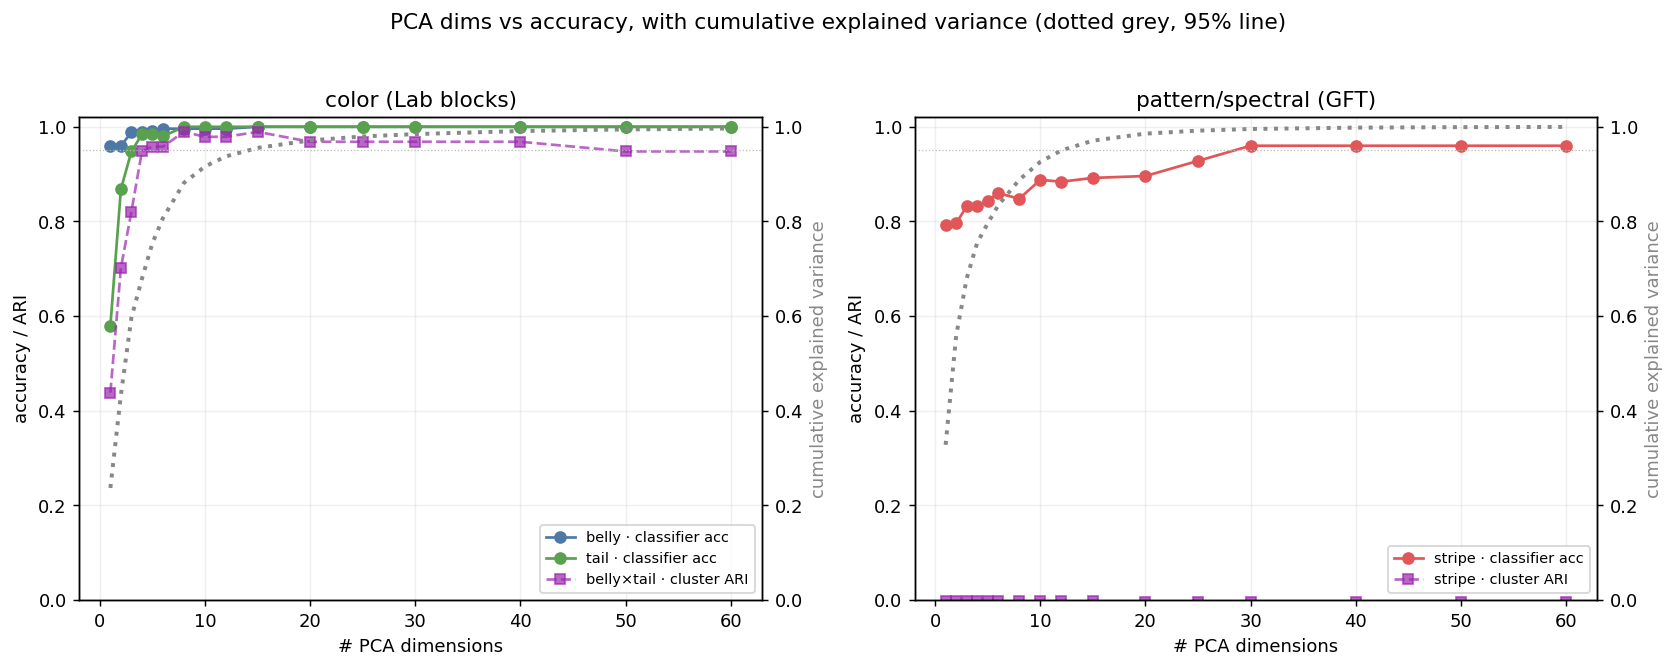
\includegraphics[width=0.95\linewidth]{dims_vs_accuracy.png}
  \caption{Accuracy vs.\ PCA dimensions, with cumulative explained variance (dotted). \emph{Left:} colour
  classification saturates by $\sim$4 dims; the belly$\times$tail clustering ARI is high. \emph{Right:} stripe
  accuracy needs $\sim$30 dims --- well past the 95\%-variance line ($\sim$12) --- so a variance criterion
  drops it; and stripe never \emph{clusters} (purple $\approx 0$ everywhere). Motivates keeping $\sim$24 dims
  and treating stripe as a supervised, not unsupervised, target.}
  \label{fig:dims}
\end{figure}

\section{The unsupervised wall: discovery is not measurement}
\label{sec:wall}

A better descriptor raises the \emph{supervised} ceiling but does not make subtle structure
\emph{discoverable}. Across PCA, ICA, UMAP, projection pursuit, and density clustering, the result is the same:
a variance-driven morphospace surfaces only factors with large between-specimen variance. Stripe (4-vs-5 under
position jitter, 80/20) has essentially \emph{no density gap} --- the optimal projection's dip statistic sits
at the noise floor --- so it is recoverable by a classifier ($\approx\!0.9$) yet invisible to clustering
($\text{ARI}\approx 0$). The rare cheeks class ($n{=}14$) is below the count that forms a significant mode at
all. This is not a defect of our pipeline; it is the expected behaviour of high-dimension--low-sample-size
(HDLSS) ``spiked covariance'' geometry: when a factor's variance is below the per-face noise variance, the
leading eigenvector rotates away from it. \emph{Supervised-recoverable but not unsupervised-discoverable} is
predictable in advance.

The honest engineering response is a \textbf{trustworthy gate} that finds real structure and refuses to invent
it. Combining a SigClust Gaussian-null test, a covariance-preserving consensus null, and per-cluster bootstrap
stability, the pipeline confirms the colour clusters (ARI 0.99 at $n{=}250$; 0.83 at $n{=}40$) and
\emph{correctly abstains} on the pattern descriptor at $n{=}40$ rather than reporting spurious groups. On the
real mussels the gate likewise reports a continuous ring-contrast gradient, not fake clusters. A morphospace
you can publish from is one that knows what it cannot see --- which is precisely why, for the subtle factors,
we turn to the expert.

\section{Expert tag-supervision breaks the ceiling}
\label{sec:tag}

If the structure is real but not density-discoverable, a small amount of supervision is the lever. We evaluated
several human-in-the-loop channels (pairwise must-link/cannot-link constraints, anchor-and-rank triplet
feedback, spring-energy morphospace morphing; see Appendix~E) and found two robust facts. First, a genuinely
overlapping low-variance factor \textbf{cannot be separated in a 2-D layout at all} --- even an oracle ranking
by true stripe count caps at $\sim$0.56 neighbourhood purity in 2-D, because 2-D has no room for it. Second,
\textbf{multi-label tagging is markedly more label-efficient than pairwise feedback}: the expert creates
named tags (``green tail'', ``5 stripes'') and clicks the specimens that have them, then a per-tag classifier
\emph{places} every unlabelled specimen and the population is laid out by the classifier's own latent.

Figure~\ref{fig:models} compares classifier families for this ``placement'' job. A \textbf{simple per-tag
linear logistic} model is the best placer --- it reaches 8-way ARI~0.86 at 80 tagged specimens (about the same
recovery that needed $\sim$200--400 \emph{pairs} via constraint feedback) and per-factor accuracy 0.93 at just
40 tags. Prototype/NCM is a close, tiny-budget-robust second; semi-supervised label propagation and learned 2-D
embeddings \emph{under}-perform, because the raw-descriptor neighbourhood graph is dominated by colour, so
labels propagate along the wrong manifold. The factors are close to linearly separable in the 24-PC space, so
the linear model both places best and keeps the demo fast and interpretable.

\begin{figure}[H]
  \centering
  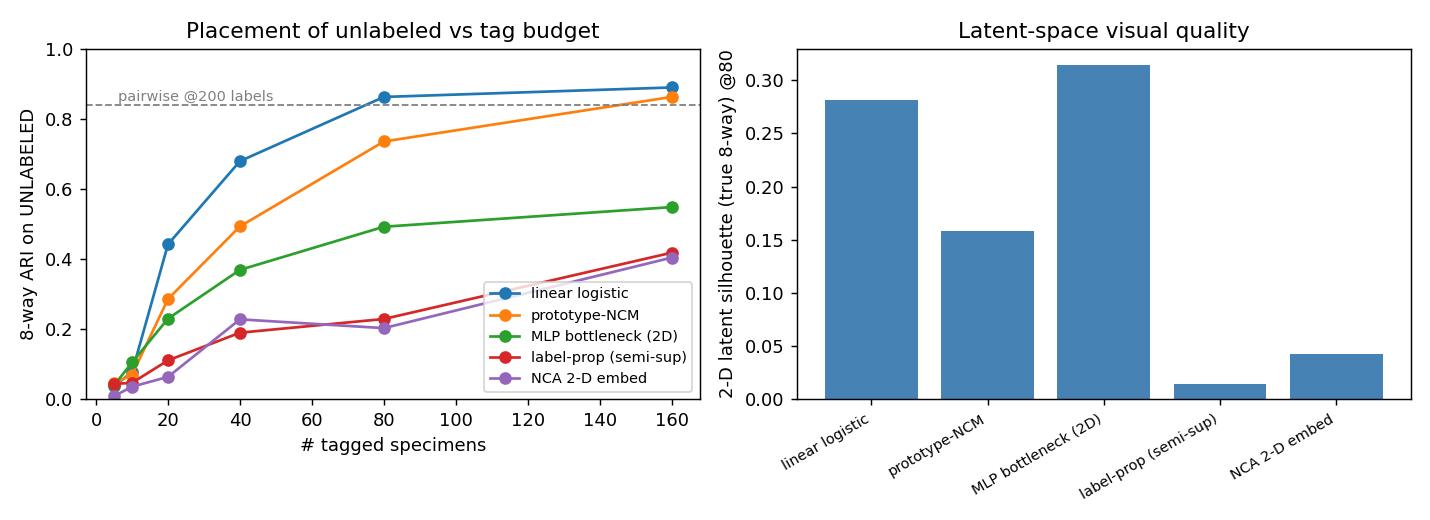
\includegraphics[width=0.97\linewidth]{model_comparison.png}
  \caption{Choosing the classifier behind tag mode. \emph{Left:} placement quality (8-way ARI on the
  \emph{unlabelled}) vs.\ tag budget --- a per-tag linear logistic model leads and matches, at 80 tags, the
  recovery that pairwise feedback reached only at $\sim$200 labels (dashed). \emph{Right:} 2-D latent
  visual quality; the linear model's latent is nearly as clean as a purpose-built 2-D bottleneck while placing
  far better.}
  \label{fig:models}
\end{figure}

The classifier defines the latent; we still have to \emph{display} it. The tag-score latent projected with
\textbf{UMAP} roughly doubles the visual separation of a PCA projection (8-way silhouette 0.57 vs.\ 0.37 at
80 tags; Fig.~\ref{fig:umap}). Crucially, UMAP on the \emph{raw} descriptor with no tags shows no structure at
all (silhouette $-0.07$): the tags-then-classifier step is what \emph{creates} the structure; UMAP only lays it
out. Because UMAP is stochastic and we want the map to react after every batch without teleporting, we re-fit it
each batch \emph{warm-started} from the previous embedding (init $=$ previous layout, $\sim$60 epochs). This is
$\sim$2.5$\times$ steadier than a naive re-fit, reacts from the very first batch, and needs no GPU or extra
dependency --- a parametric-UMAP encoder is marginally smoother but pulls in TensorFlow, and offline aligned-UMAP
is far too slow for live use.

\begin{figure}[H]
  \centering
  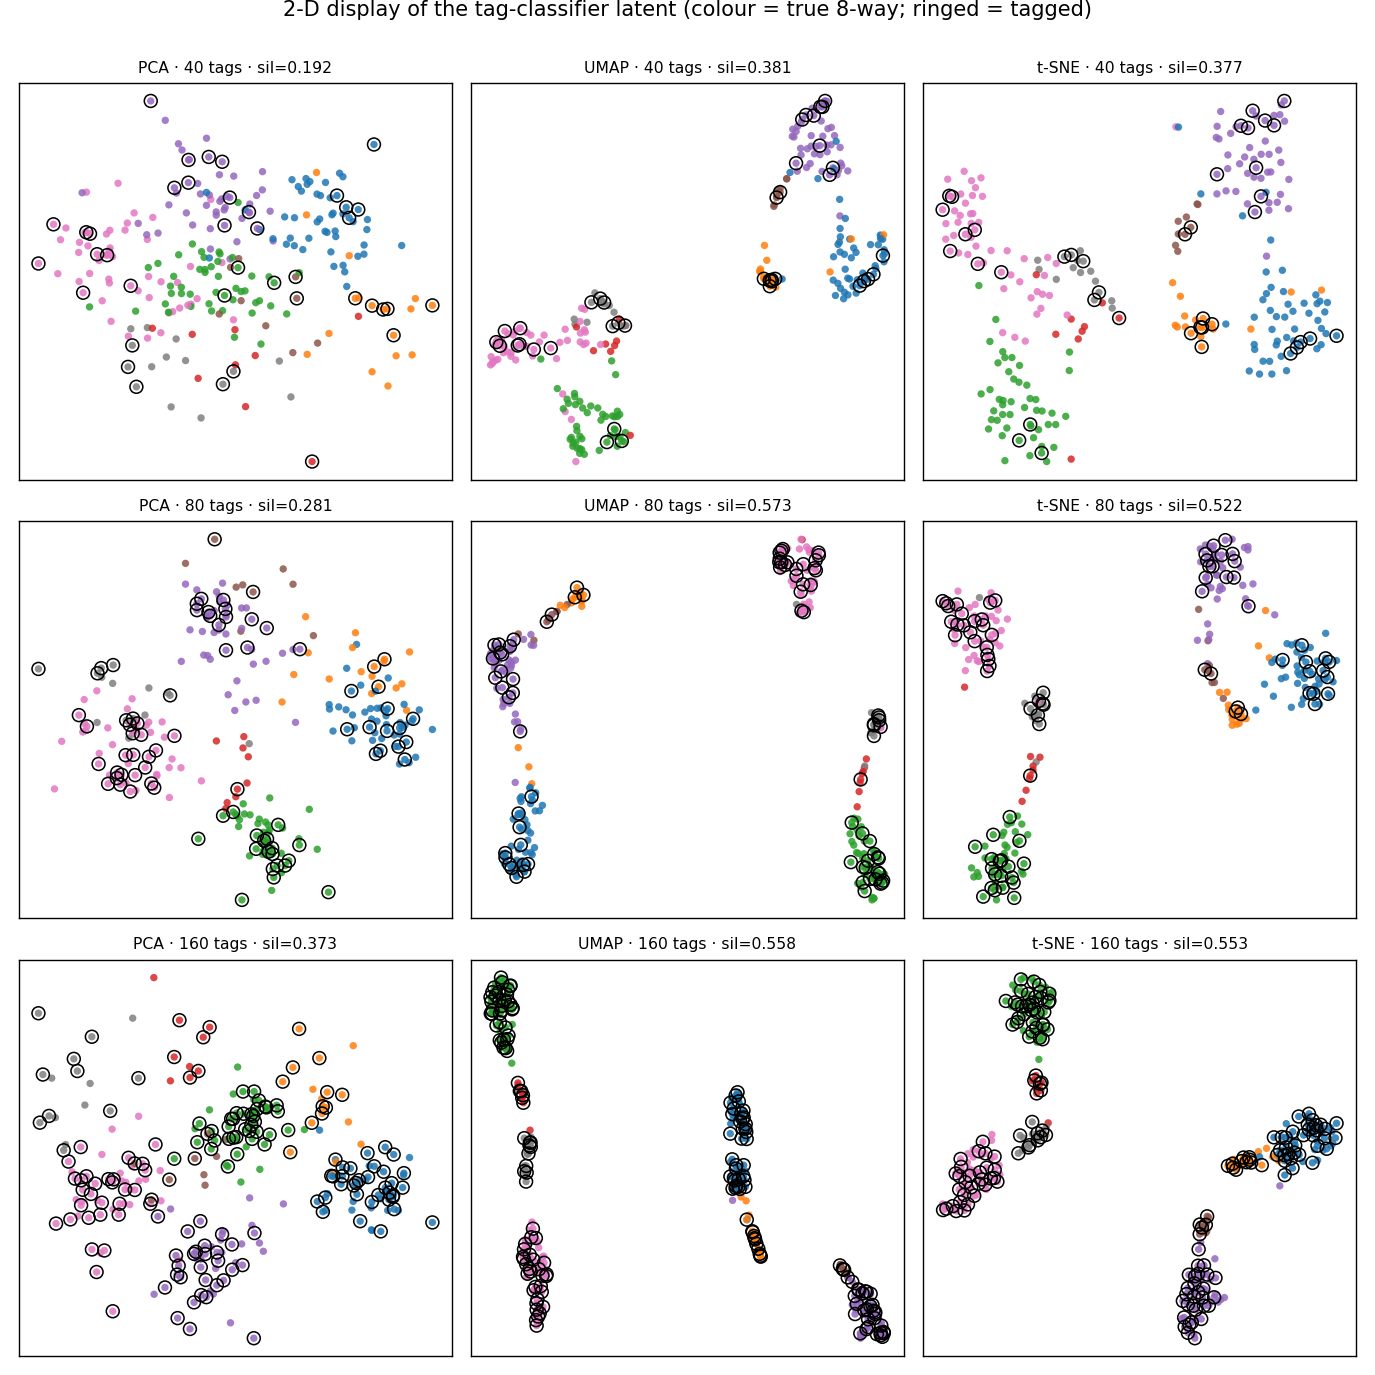
\includegraphics[width=0.62\linewidth]{umap_latent_compare.png}
  \caption{Displaying the tag-classifier latent in 2-D (rows: 40/80/160 tags; columns: PCA, UMAP, t-SNE;
  colour $=$ true 8-way group). UMAP (and t-SNE) resolve the groups into clean islands where PCA stays a muddy
  blob. The structure comes from the tags; the projection only arranges it.}
  \label{fig:umap}
\end{figure}

\paragraph{Active learning and the rare class.} Two more choices follow from the data. After each applied
batch the tool \emph{auto-rolls} the next batch by \textbf{uncertainty} (the unlabelled specimens whose per-tag
predictions are nearest 0.5); this beats random selection decisively (8-way ARI 0.96 vs.\ 0.81 at 80 labels;
Fig.~\ref{fig:active}, left). But uncertainty sampling is a poor way to \emph{first} encounter a rare class. For
cold start we seed the very first batch by \textbf{novelty} --- mean $k$-nearest-neighbour distance in the
compressed PCA space --- which surfaces the first rare ``cheeks'' specimen at rank~1 versus $\sim$16 random
labels, a 10--16$\times$ speedup (Fig.~\ref{fig:active}, right). Novelty/anomaly scoring surfaces any
\emph{separable} minority (it does nothing for an arbitrary random rare subset), and only in the compressed
space --- distance-based anomaly collapses in the raw 640-D colour descriptor. Finally, the per-tag logistic
uses \code{class\_weight='balanced'}, which adds $\approx\!0.09$ balanced accuracy for the rare factors in the
early regime and ties SMOTE/ADASYN without the dependency.

\begin{figure}[H]
  \centering
  \begin{minipage}[c]{0.46\linewidth}\centering
    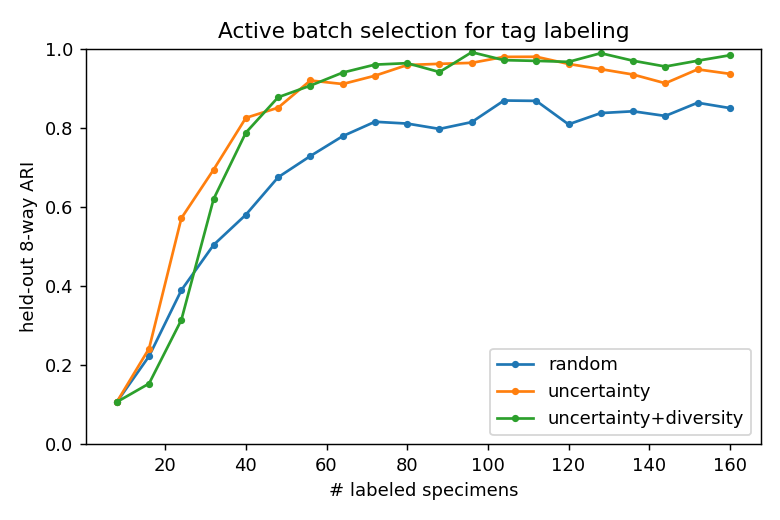
\includegraphics[width=\linewidth]{active_tags.png}
  \end{minipage}\hfill
  \begin{minipage}[c]{0.50\linewidth}\centering
    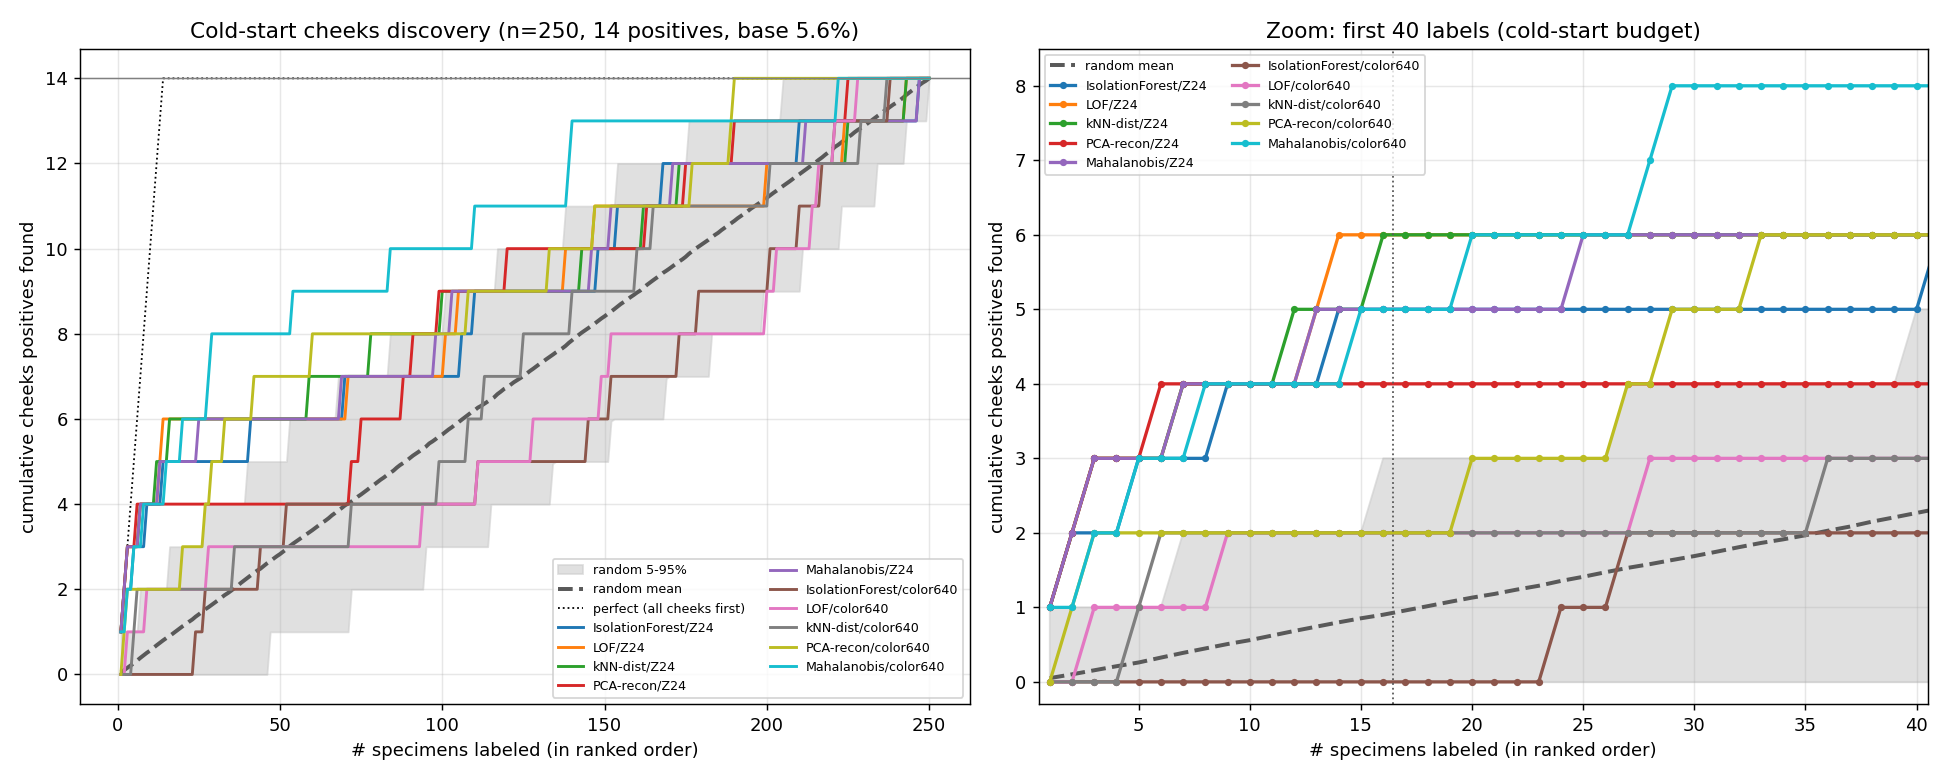
\includegraphics[width=\linewidth]{coldstart_discovery.png}
  \end{minipage}
  \caption{\emph{Left:} after each batch, auto-rolling the next batch by classifier uncertainty $\gg$ random
  selection. \emph{Right:} cold-start novelty seeding finds rare-class members an order of magnitude faster
  than random for the first few labels (then hands off to uncertainty sampling).}
  \label{fig:active}
\end{figure}

\section{The expert-tagging tool}
\label{sec:tool}

These findings assemble into a single interactive tool (Fig.~\ref{fig:demo}). The expert explores batches of
specimens, creates trait tags, selects an active tag and clicks the specimens that show it (multi-label), and
hits \emph{Apply}; the tool retrains the per-tag classifier and updates a 2-D morphospace and a clustering tree
of the classifier latent. It then auto-rolls the next, most-informative batch. A frontend-only static build
runs entirely in the browser for sharing.

\begin{table}[H]
  \centering
  \small
  \caption{What landed in the tool, and the experiment that justifies it.}
  \label{tab:choices}
  \begin{tabular}{p{0.30\linewidth} p{0.40\linewidth} p{0.24\linewidth}}
    \toprule
    Choice & Why & Rejected alternative \\
    \midrule
    Per-region colour+texture $\rightarrow$ PCA-24 & subtle factors live in the low-variance tail; $\sim$24--30 dims keeps them & EV-threshold ($\sim$12 dims, drops stripe) \\
    Per-tag linear logistic, $C{=}0.5$ & best placer; near-linearly separable; fast \& interpretable & MLP / label-prop / NCA (worse placement) \\
    \code{class\_weight='balanced'} & free $+0.09$ for rare tags early & SMOTE/ADASYN (tie, extra dep.) \\
    Warm-started UMAP of tag latent & doubles separation over PCA; smooth, reactive, no GPU & PCA (muddy); parametric (TF); aligned (slow) \\
    Uncertainty auto-roll & $\gg$ random ($0.96$ vs $0.81$) & random / uncertainty+diversity (worse early) \\
    Cold-start novelty seed & 10--16$\times$ faster first rare-class hit & NN-expansion / raw-space anomaly (fail) \\
    Ward tree on the latent & label-free overview of recovered groups & --- \\
    Multi-label tagging & far more label-efficient than pairwise; direct predictions & pairwise / triplet / spring (2-D ceiling) \\
    \bottomrule
  \end{tabular}
\end{table}

\begin{figure}[H]
  \centering
  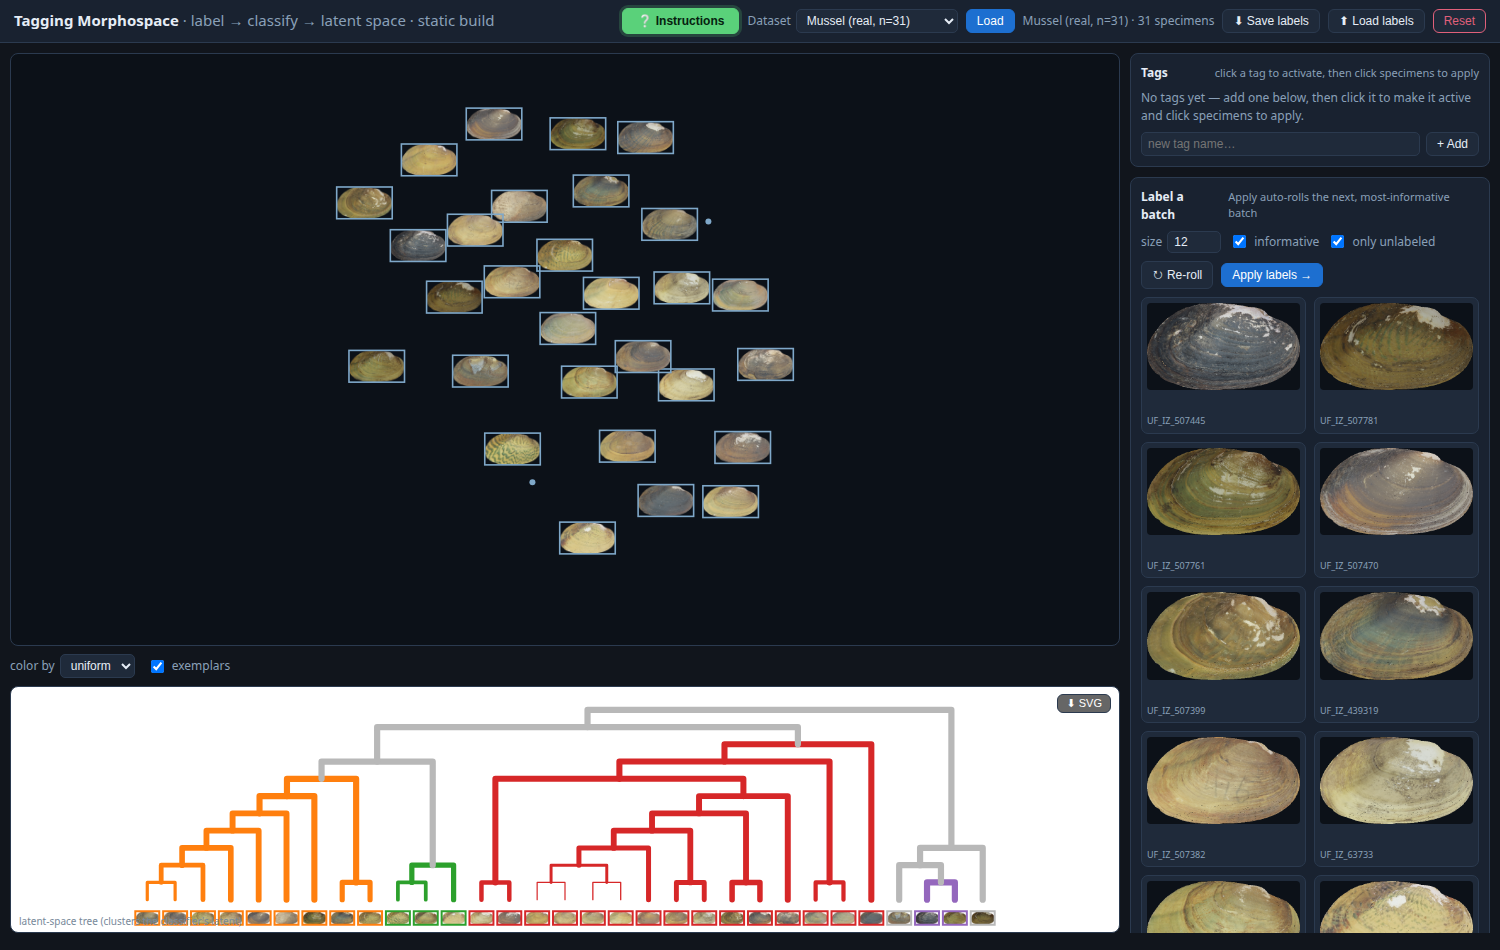
\includegraphics[width=0.92\linewidth]{demo_screenshot.png}
  \caption{The expert-tagging tool (here on the real mussel valves). Left: the classifier-latent morphospace
  with specimen exemplars and a clustering tree; right: the tag palette and the batch the expert is labelling.
  Tag, Apply, and the next informative batch rolls automatically.}
  \label{fig:demo}
\end{figure}

\section{Discussion and limitations}

The arc is the message: a colour morphospace solves what is easy; a general spectral/texture descriptor makes
pattern \emph{recoverable}; but recoverable is not the same as \emph{discoverable}, and on small real
populations the honest unsupervised answer is often ``a colour split and a continuous gradient, nothing more.''
A few minutes of expert tagging converts the supervised-only structure into a navigable, predicted morphospace
at a fraction of the labelling effort of pairwise feedback. Honest limits remain: the rare cheeks class plateaus
near $\approx\!0.66$ balanced accuracy in the tool's 24-dimensional representation even given all positives
($\approx\!0.79$ with the richest descriptor; 14 examples is simply few), and a truly
overlapping factor shows as a gradient, not a cluster, in any 2-D view --- so the tool's value is that you can
\emph{see and label} such structure, not that it auto-separates. The methods are CPU-only and transfer to real
data (mussels) and to different meshes (the spectral descriptor is topology-independent). A condensed ledger of
all experiments follows.

\appendix
\section*{Appendix: condensed experiment ledger}
\addcontentsline{toc}{section}{Appendix}
\renewcommand{\thesubsection}{\Alph{subsection}}

\small

\subsection{Problem framing \& baseline (EXP-00,01,04,05)}
Verified the planted ground truth (belly/tail independent; stripe 79/21; cheeks 5.6\%). Reproduced the module's
colour morphospace: belly/tail $\approx\!1.0$, stripe 0.5--0.75, cheeks $\approx$ chance. Established the
governing principle --- \emph{discovery $\neq$ measurement}: variance-driven reduction shows only high-variance
factors; subtle structure must be measured/supervised. End-to-end ``recommended'' pipeline: colour clusters
(ARI 0.99) + a measured stripe axis (0.64$\rightarrow$0.89) + a rare-variant flag.

\subsection{Pattern descriptors (EXP-02,03,07,20,22,25,27,30,53,54)}
Hand-tuned axial band-count detector (0.88, but taxon-specific) $\rightarrow$ \emph{general} graph-spectral
band energy $\rightarrow$ \textbf{signed GFT coefficients} ($k{=}40$; stripe 0.93, cheeks 0.77; the best single
general descriptor) $\rightarrow$ \textbf{shared-codebook texton BoW} (stripe 0.97, the best on fishy).
Segmentation$+$spatial/Endler ties GFT and adds interpretable arrangement stats. Both descriptors measure
\emph{count}, not the spacing/width confound (supervised direction correlates $|r|\gtrsim 0.95$ with count
--- GFT 0.99, segmentation 0.95 --- and $\lesssim 0.03$ with spacing). \emph{Negative result:} segment-then-GFT is worse than either alone --- do not chain them.
Dimension/mode sweeps: keep $\sim$24 PCA dims / $k\!\gtrsim\!40$ modes; explained variance mis-sizes both.

\subsection{The unsupervised wall \& trustworthy gating (EXP-11,12,13--15,32,38--41)}
Mapped what unsupervised discovery can honestly reach: well-separated balanced clusters (belly/tail) YES;
subtle overlapping structure (stripe) NO (no density gap; dip $\approx$ noise floor); rare minority (cheeks,
$n{=}14$) NO; genuinely continuous variation $\rightarrow$ the gate ABSTAINS. The HDLSS reframing (Jung--Marron
spiked covariance) makes this predictable in advance. A SigClust $+$ consensus-null $+$ bootstrap-Jaccard gate
finds the colour structure (ARI 0.99/0.83 at $n{=}250/40$) and abstains on pattern at $n{=}40$. Localized,
per-region gated clustering and covariation-based mesh parcellation auto-isolate the colour modules and emit a
label-free ``structure map,'' but still cannot cluster the subtle/rare factors.

\subsection{Representation, dimensionality, imbalance (EXP-53,54,55,56,57,59)}
Subtle factors sit in the low-variance PCA/spectral tail, so keep generous dimensionality. ICA $\equiv$ PCA for
linear classifiers (not a recovery lever), though ICA cleanly isolates the strong colour factors for
interpretability. For class imbalance, \code{class\_weight='balanced'} $\approx$ SMOTE $\approx$ ADASYN --- the
binding constraint is the minority \emph{count}, not the loss machinery --- so use the free reweighting.

\subsection{Expert-in-the-loop supervision (EXP-29,33,34,35,36,37,42--45)}
Plain few-label supervision and label propagation are label-inefficient on a generic high-dim descriptor.
Pairwise constraint metric-warping recovers stripe (ARI 0$\rightarrow$0.42 at 80 pairs); anchor-and-rank
triplet feedback sharpens whatever trait the expert ranks (``you get what you rank''); a spring-energy
morphospace gives a faithful interactive morph. Two robust lessons: a low-variance overlapping factor has a hard
\emph{2-D ceiling} ($\sim$0.56 even with an oracle ranking), and diverse panels aid exploration while
\emph{local} panels aid fine discrimination. Recovering the full $2^3{=}8$-cluster structure needs graded target
distances $+$ a low-rank metric $+$ clustering in the 24-D space (ARI $\approx 0.84$ at 200 labels), shown as a
factor grid rather than hoping 2-D springs separate eight groups.

\subsection{The tagging tool (EXP-46--52,58,60)}
Multi-label tagging beats pairwise feedback for label efficiency and yields direct predictions. Best placer $=$
per-tag linear logistic in 24-PC space (8-way ARI 0.86 at 80 tags); semi-supervised/embedding models
under-perform. Display $=$ \textbf{warm-started UMAP} of the tag-score latent (doubles PCA's separation;
reactive from batch~1; no TF). Active \textbf{uncertainty} auto-roll $\gg$ random; \textbf{cold-start novelty}
seeding finds rare-class members 10--16$\times$ faster; anomaly scoring surfaces any \emph{separable} minority,
in the compressed space only. Net build: per batch $=$ retrain six linear tag classifiers (ms) $+$ a
warm-started UMAP fit ($\sim$0.2\,s at $n{=}250$) $\rightarrow$ client tweens to the new coordinates.

\subsection{Generality / real data (EXP-08,09,10,21,28,40,41)}
The same engine transfers to the real mussel valves (different mesh, baking artefacts) and to a charisma-style
phenetic dendrogram with mesh-rendered exemplars: it produces an interpretable colour split and a continuous
ring-contrast pattern axis, and the gate correctly abstains from inventing discrete pattern clusters --- the
behaviour we want when ground truth is unavailable.

\end{document}
